\documentclass{beamer}
\usepackage[utf8]{inputenc}
\usepackage[spanish]{babel}
\usepackage[T1]{fontenc}
\usepackage{graphicx}
\usepackage{mathptmx}
\usepackage{helvet}
\usepackage{color}
\usepackage{tikz}

%--------------------------------------------------------------------------------------------------
%                                   DATOS PARA LA PORTADA
%--------------------------------------------------------------------------------------------------
\title{Aplicaciones nanométricas y cuánticas \\de 
ecuaciones diferenciales no lineales asociadas a lineales}
\date{\today}
\author[Vic]{M. en C. Victor Hugo Carrera Escobedo} %\texttt{hadron\_n@hotmail.com}}
%--------------------------------------------------------------------------------------------------

%--------------------------------------------------------------------------------------------------
%                                             TEMA
%--------------------------------------------------------------------------------------------------
\usetheme{texsx}
%--------------------------------------------------------------------------------------------------


\begin{document}

%--------------------------------------------------------------------------------------------------
%			Página de Título
%--------------------------------------------------------------------------------------------------


\begin{frame}
\titlepage
\end{frame}

%--------------------------------------------------------------------------------------------------
%			Introducción
%--------------------------------------------------------------------------------------------------

\begin{frame}
\frametitle{Antecedentes}
\framesubtitle{Ecs. no lineales asociadas a lineales}

\begin{itemize}
 \item Sturm-Liouville.
 \item Riccati
 \item Ermakov
\end{itemize}

\end{frame}



\begin{frame}
\frametitle{Antecedentes}
\framesubtitle{Aplicaciones}
\begin{columns}
\column{0.3\textwidth}
Ermakov
\begin{itemize}
 \item Osciladores amortiguados.
 \item Óptica no lineal.
 \item Mecánica cuántica.
 \item Óptica cuántica.
\end{itemize}

\column{0.3\textwidth}
Riccati
\begin{itemize}
 \item Termo.
 \item Socio-física.
 \item Econo-física.
 \item Elastomecánica.
\end{itemize}

\column{0.3\textwidth}
Matriz de transferencia
\begin{itemize}
 \item Propagación de ondas.
 \item Invisivilidad.
 \item Cristales fotónicos.
 \item Amarre fuerte.
\end{itemize}

\end{columns}
\end{frame}

\begin{frame}
\frametitle{Metodología}
\framesubtitle{Método de la matriz de transferencia}

\end{frame}

\begin{frame}
\frametitle{Metodología}
\framesubtitle{Ecuación de Riccati}

Buscar rayos X + Riccati

\end{frame}

\begin{frame}
\frametitle{Metodología}
\framesubtitle{MMT basado en Riccati}

\end{frame}

\begin{frame}
\frametitle{Metodología}
\framesubtitle{Procedimiento Lewis-Ermakov}

\end{frame}

\begin{frame}
\frametitle{Objetivos}
\framesubtitle{Generales}
\begin{enumerate}
 \item Adquirir una base sólida de ecuaciones diferenciales no lineales.
 \item Analizar las aplicaciones actuales de los sistemas tipo Ermakov/Riccati.
 \item Crear conexiones entre estos sistemas y la física de materiales.
 \item Generar contenido científico en base a lo anterior.
\end{enumerate}
\end{frame}

\begin{frame}
\frametitle{Metas}
\framesubtitle{Pautas a tener en cuenta}
\begin{itemize}
 \item Adquirir las bases de ecuaciones diferenciales no lineales.
 \item Revisión bibliográfica.
 \item Analizar al menos un tema o aplicación de sistemas no lineales por semestre.
 \item Modelar matemáticamente el sistema.
 \item Generar códigos computacionales que permitan analizar las propiedades del sistema bajo
 distintos parámetros físicos.
 \item Crear contenido científico publicable en revistas arbitradas.
 \item Recopilar la información anterior para escribir una tesis a manera de coloquio.
\end{itemize}
\end{frame}

\begin{frame}
\frametitle{Programa de actividades}
\framesubtitle{Cronograma}

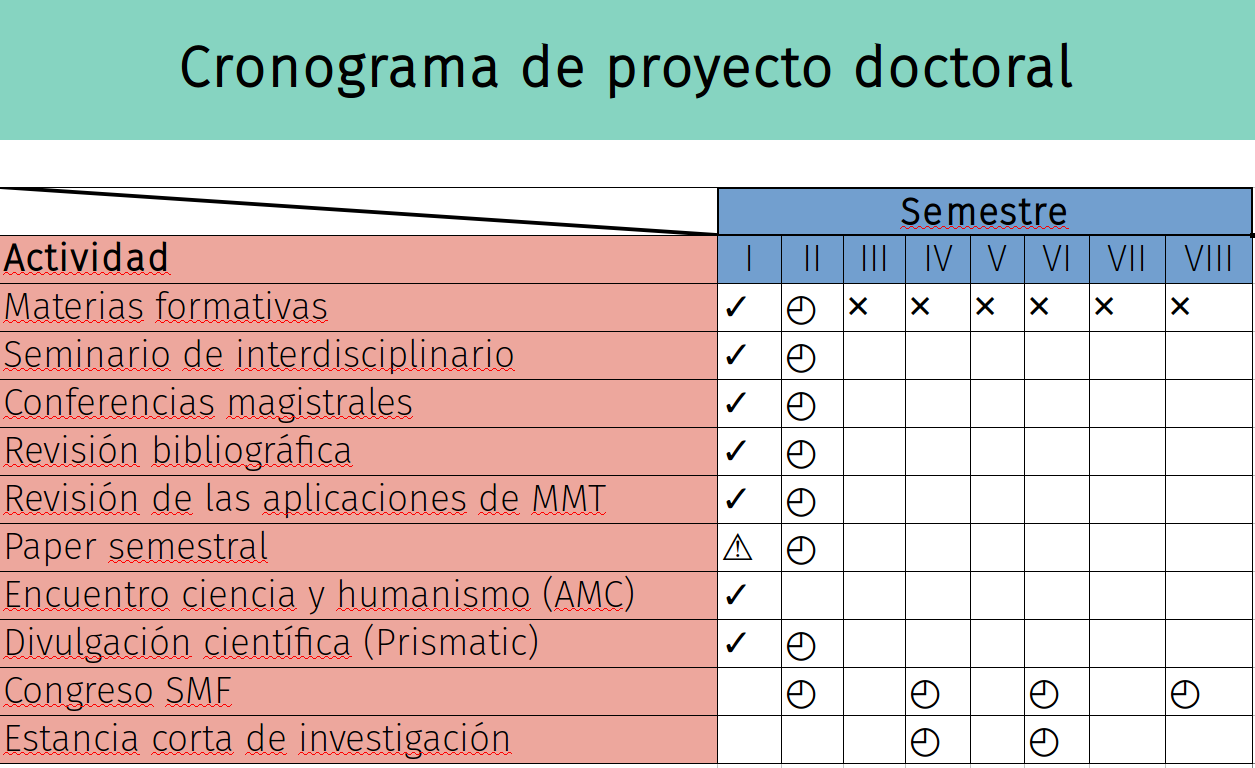
\includegraphics[width=\textwidth]{img/crono.png}

\end{frame}



% \begin{frame}
% \frametitle{Título}
% \framesubtitle{Subtítulo}
% \begin{columns}
%  \column{0.5\textwidth}
%   \includegraphics[width=1.1\textwidth]{}
%  \column{0.5\textwidth}
%   \begin{itemize}
%   \item 
%  \end{itemize}
% \end{columns}
% \footnote{Pie de slide algo}
% \end{frame}




% \begin{frame}
% \frametitle{título}
% \framesubtitle{sub}
% \begin{itemize}
%  \item 
% \end{itemize}
% 
% \end{frame}
% 
% \begin{frame}[plain]
% \setlength{\unitlength}{1 cm}
% \begin{picture}(1,1)
% \put(-3,-5.7){\includegraphics[]{}
% \end{picture}
% \end{frame}



% \begin{frame} 
% \frametitle{Título de Slide 1} 
% \framesubtitle{Subtítulo del Slide: \textit{itálicas}} 
% \begin{theorem}
% There is no largest prime number. \end{theorem} 
% \begin{enumerate} 
% \item<1-| alert@1> Suppose $p$ were the largest prime number. 
% \item<2-> Let $q$ be the product of the first $p$ numbers. 
% \item<3-> Then $q+1$ is not divisible by any of them. 
% \item<4-> But $q + 1$ is greater than $1$, thus divisible by some prime
% number not in the first $p$ numbers.
% \end{enumerate}
% \end{frame}

% \begin{frame}%{A longer title}
% \frametitle{Título de Slide}
% \framesubtitle{Subtítulo }
% 
% \transwipe
% \begin{itemize}
% \item one
% \item two
% \end{itemize}
% \end{frame}


\end{document}